% Credits are indicated where needed. The general idea is based on a template by Vel (vel@LaTeXTemplates.com) and Frits Wenneker.

\documentclass[11pt, a4paper]{article} % General settings in the beginning (defines the document class of your paper)
% 11pt = is the font size
% A4 is the paper size
% “article” is your document class

%----------------------------------------------------------------------------------------
%	Packages
%----------------------------------------------------------------------------------------

% Necessary
\usepackage[german,english]{babel} % English and German language 
\usepackage{booktabs} % Horizontal rules in tables 
% For generating tables, use “LaTeX” online generator (https://www.tablesgenerator.com)
\usepackage{comment} % Necessary to comment several paragraphs at once
\usepackage[utf8]{inputenc} % Required for international characters
\usepackage[T1]{fontenc} % Required for output font encoding for international characters

% Might be helpful
\usepackage{amsmath,amsfonts,amsthm} % Math packages which might be useful for equations
\usepackage{tikz} % For tikz figures (to draw arrow diagrams, see a guide how to use them)
\usepackage{tikz-cd}
\usetikzlibrary{positioning,arrows} % Adding libraries for arrows
\usetikzlibrary{decorations.pathreplacing} % Adding libraries for decorations and paths
\usepackage{tikzsymbols} % For amazing symbols ;) https://mirror.hmc.edu/ctan/graphics/pgf/contrib/tikzsymbols/tikzsymbols.pdf 
\usepackage{blindtext} % To add some blind text in your paper
\usepackage{listings}
\usepackage{color}

\definecolor{dkgreen}{rgb}{0,0.6,0}
\definecolor{gray}{rgb}{0.5,0.5,0.5}
\definecolor{mauve}{rgb}{0.58,0,0.82}

\lstset{frame=tb,
  language=Java,
  aboveskip=7mm,
  belowskip=5mm,
  showstringspaces=false,
  columns=flexible,
  basicstyle={\small\ttfamily},
  numbers=none,
  numberstyle=\tiny\color{gray},
  keywordstyle=\color{blue},
  commentstyle=\color{dkgreen},
  breaklines=true,
  breakatwhitespace=false,
  tabsize=3
}


%---------------------------------------------------------------------------------
% Additional settings
%---------------------------------------------------------------------------------

%---------------------------------------------------------------------------------
% Define your margins
\usepackage{geometry} % Necessary package for defining margins

\geometry{
	top=2cm, % Defines top margin
	bottom=2cm, % Defines bottom margin
	left=2.2cm, % Defines left margin
	right=2.2cm, % Defines right margin
	includehead, % Includes space for a header
	%includefoot, % Includes space for a footer
	%showframe, % Uncomment if you want to show how it looks on the page 
}

\setlength{\parindent}{15pt} % Adjust to set you indent globally 

%---------------------------------------------------------------------------------
% Define your spacing
\usepackage{setspace} % Required for spacing
% Two options:
\linespread{1.5}
%\onehalfspacing % one-half-spacing linespread

%----------------------------------------------------------------------------------------
% Define your fonts
\usepackage[T1]{fontenc} % Output font encoding for international characters
\usepackage[utf8]{inputenc} % Required for inputting international characters

\usepackage{XCharter} % Use the XCharter font


%---------------------------------------------------------------------------------
% Define your headers and footers

\usepackage{fancyhdr} % Package is needed to define header and footer
\pagestyle{fancy} % Allows you to customize the headers and footers

%\renewcommand{\sectionmark}[1]{\markboth{#1}{}} % Removes the section number from the header when \leftmark is used

% Headers
\lhead{} % Define left header
\chead{\textit{}} % Define center header - e.g. add your paper title
\rhead{} % Define right header

% Footers
\lfoot{} % Define left footer
\cfoot{\footnotesize \thepage} % Define center footer
\rfoot{ } % Define right footer

%---------------------------------------------------------------------------------
%	Add information on bibliography
\usepackage{natbib} % Use natbib for citing
\usepackage{har2nat} % Allows to use harvard package with natbib https://mirror.reismil.ch/CTAN/macros/latex/contrib/har2nat/har2nat.pdf

% For citing with natbib, you may want to use this reference sheet: 
% http://merkel.texture.rocks/Latex/natbib.php

%---------------------------------------------------------------------------------
% Add field for signature (Reference: https://tex.stackexchange.com/questions/35942/how-to-create-a-signature-date-page)
\newcommand{\signature}[2][5cm]{%
  \begin{tabular}{@{}p{#1}@{}}
    #2 \\[2\normalbaselineskip] \hrule \\[0pt]
    {\small \textit{Signature}} \\[2\normalbaselineskip] \hrule \\[0pt]
    {\small \textit{Place, Date}}
  \end{tabular}
} % Loads required packages from the separate file 

%---------------------------------------------------------------------------------
%	General information
%---------------------------------------------------------------------------------
\title{Quarterback Safety in American Football} % Adds your title


\author{
FIRSTNAME LASTNAME % Add your first and last name
    %\thanks{} % Adds a footnote to your title
    %\institution{YOUR INSTITUTION} % Adds your institution
  }

% \date{\small \today} % Adds the current date to your “cover” page; leave empty if you do not want to add a date


%---------------------------------------------------------------------------------
%	Define what’s in your document
%---------------------------------------------------------------------------------

\begin{document}

% If you want a cover page, uncomment "%---------------------------------------------------------------------------------
% Cover page
%---------------------------------------------------------------------------------

% Here are more templates for other cover pages: https://www.latextemplates.com/cat/title-pages

% This example is based on this cover page example: https://www.latextemplates.com/template/academic-title-page

\begin{titlepage} % Starts new environment where the page number is not displayed and the count starts at 1 for the next page

%------------------------------------------------
%	Institutional information
%------------------------------------------------
	
\begin{minipage}{0.8\textwidth} % Begins new environment (like a text box)
    \begin{flushleft} % Sets environment on the left side of the paper
    \large
    Carnegie Mellon University\\ % Add your institution
    Fall 2020\\ % Add term
    \end{flushleft}
\end{minipage}
	
\vspace*{2in} % Adds some space in-between
	
\center % Centre everything on the page

%------------------------------------------------
%	Main part
%------------------------------------------------
	
{\Huge\bfseries Quarterback Safety In American Football}\\[0.4cm] % Add your paper title 
{\huge \textit{Modeling the Sport of American Football \\ through the Lens of a Hybrid System}}\\

\vfill

{\large December 13, 2020}\\[0.4cm] % Add date (current day)
Len Huang \texttt{(lghuang)}\\ % Add your name
Megha Jain \texttt{(meghaj2)}\\

\vfill

{ \large Term Paper } \\
\textbf{15-424:} Logical Foundations of Cyber-Physical Systems\\ % Add course title
\textbf{Instructor:} Andr\'e Platzer\\
\textbf{Teaching Assistant:} Jonathan Laurent
	
\vfill % Adds additional space


	

	
\end{titlepage}" and comment "\maketitle" as well as "\begin{center} % Center text
    Word count: XXXX
% How to check words in a LaTeX document: https://www.overleaf.com/help/85-is-there-a-way-to-run-a-word-count-that-doesnt-include-latex-commands
\end{center}"

% \maketitle % Print your title, author name and date; comment if you want a cover page 
%---------------------------------------------------------------------------------
% Cover page
%---------------------------------------------------------------------------------

% Here are more templates for other cover pages: https://www.latextemplates.com/cat/title-pages

% This example is based on this cover page example: https://www.latextemplates.com/template/academic-title-page

\begin{titlepage} % Starts new environment where the page number is not displayed and the count starts at 1 for the next page

%------------------------------------------------
%	Institutional information
%------------------------------------------------
	
\begin{minipage}{0.8\textwidth} % Begins new environment (like a text box)
    \begin{flushleft} % Sets environment on the left side of the paper
    \large
    Carnegie Mellon University\\ % Add your institution
    Fall 2020\\ % Add term
    \end{flushleft}
\end{minipage}
	
\vspace*{2in} % Adds some space in-between
	
\center % Centre everything on the page

%------------------------------------------------
%	Main part
%------------------------------------------------
	
{\Huge\bfseries Quarterback Safety In American Football}\\[0.4cm] % Add your paper title 
{\huge \textit{Modeling the Sport of American Football \\ through the Lens of a Hybrid System}}\\

\vfill

{\large December 13, 2020}\\[0.4cm] % Add date (current day)
Len Huang \texttt{(lghuang)}\\ % Add your name
Megha Jain \texttt{(meghaj2)}\\

\vfill

{ \large Term Paper } \\
\textbf{15-424:} Logical Foundations of Cyber-Physical Systems\\ % Add course title
\textbf{Instructor:} Andr\'e Platzer\\
\textbf{Teaching Assistant:} Jonathan Laurent
	
\vfill % Adds additional space


	

	
\end{titlepage} % Adds a cover page; uncomment if you want a cover page
% \begin{center} % Center text
    Word count: XXXX
% How to check words in a LaTeX document: https://www.overleaf.com/help/85-is-there-a-way-to-run-a-word-count-that-doesnt-include-latex-commands
\end{center} % Gives you the word count; comment if you want a cover page 
%---------------------------------------------------------------------------------
% Table of content
%---------------------------------------------------------------------------------

\newpage % Generates page break

% Table of content
\thispagestyle{empty} % Suppresses page numbers
\tableofcontents % Adds table of content
\newpage % Generates page break

% List of figures
%\thispagestyle{empty} % Suppresses page numbers
%\listoffigures % Adds list of figures; uncomment if required
%\newpage % Generates page break; uncomment if required

% List of tables
%\thispagestyle{empty} % Suppresses page numbers
%\listoftables % Adds list of tables; uncomment if required
%\newpage % Generates page break; uncomment if required
 % Adds a table of content; uncomment if required
%---------------------------------------------------------------------------------
% Abstract
%---------------------------------------------------------------------------------

\begin{abstract}

\quad


American football lends itself to modelling in many ways and has clearly defined rules for what we will refer to as “safety” and “efficiency”. While it is not the most pressing issue in our society, modelling football can help us understand how to think of more important multi-agent systems. In the time spent developing models, we made note of many important modeling subtleties like the pass interference and maximum passing range. We also raised future questions for ways to more accurately model football with Quarterback controllers and probabilistic linemen. Finally, we found clever modelling simplifications that still preserve the safety and efficiency of the system. The approaches we took in this paper to develop our models can help us explore more advanced systems in the future.


\end{abstract} % Adds your abstract
%----------------------------------------------------------------------------------------
% Introduction
%----------------------------------------------------------------------------------------
\setcounter{page}{1} % Sets counter of page to 1

\section{Introduction} % Add a section title

\quad American football lends itself to modelling in many ways and has clearly defined rules for what we will refer to as “safety” and “efficiency”. Much work has been done with making models for fútbol / soccer, especially with events like the RoboCup. But we seek to lay the groundwork for how we might approach similar problems of modelling, with American football (to which we refer to as “football”). 

\subsection{American Football in a Nutshell}

\quad Football is played by two teams of eleven players on a rectangular field with goalposts at either end. The offense is the team that has possession of the ball. Their goal is to advance down the field by either running with or passing the ball. The defense is the team without possession of the ball. Their goal is to stop the advance of the offense. Football is played in increments. First, players line up along a line, facing each other. Then, the offense starts an “increment” by handing the ball to the quarterback. Action is continued until either the ball makes its way to the end of the field (or the endzone), or the player with the ball is stopped (often by being tackled to the ground). We will refer to a single increment as a “play”. \\ 
 
For the offensive team, there are three core roles which we will focus on: the offensive linemen (OL), quarterback (QB), and wide receiver (WR). A typical passing play in football involves the QB throwing the ball to the WR as the OL is protecting him from the defense. The QB may need to move around in order to avoid getting hit by the defense. However, the QB must avoid moving too quickly, because if he does, he will no longer be able to accurately pass to the WR. This is the prime challenge we seek to discuss in our model! But more on that later. \\ 
 
For the defensive team, there are two core roles which we will focus on: the defensive linemen (DL) and the linebacker (LB). The goal of the DL is to break past the OL in order to tackle the QB (often referred to as a “sack”) before he is able to pass the ball. The goal of the LB is to prevent the WR from catching the ball and to stop him after he catches it. One rule to note is that the LB is not allowed to touch the WR before he catches the ball, and can only indirectly influence his ability to catch the ball (block it, intercept it, etc). If he does, then it is considered a “pass interference” and counted as a violation against the defense. \\

The offense and defense generally have different strategies they follow. An offensive strategy might look like one where the wide receivers run in certain patterns or "routes". A defensive strategy might be one where linebackers are strategically placed to either prevent the ball from being caught or sack the quarterback. We will discuss an offensive strategy later, but mention two defensive strategies now: man and zone. \\ 

A man-to-man defense is one where each linebacker follows a wide receiver. This is so that the defense can essentially have a player "assigned" to each wide receiver, effectively denying them of all possible offensive opportunities. As such, whatever route the wide receiver runs, the linebacker will follow.\\

A zone defense is one where the defensive players attempt to spread themselves out evenly throughout the field, or in some sort of pattern. This is so that the defense can be in a more general position to cover the offense depending on how the wide receivers run, since they do not have access to this information. 

\subsection{Summary of Terms}

\quad Here are some terms that we will be using regularly throughout this proposal. Feel free to look back here if the terms or abbreviations get confusing. We also note some other specifics that may be necessary to know moving forward. Note that some of these positions are more nuanced in actual football, and that we restrict their responsibilities for the sake of a simpler analysis.

\begin{enumerate}
    \item \textbf{Player Roles}
        \begin{enumerate}
            \item \textbf{Quarterback (QB):} Offensive player responsible for passing the ball to WR’s
            \item \textbf{Wide Receiver (WR):} Offensive player responsible for catching the ball 
            \item \textbf{Offensive Linemen (OL):} Offensive player responsible for protecting the QB 
            \item \textbf{Defensive Lineman (DL):} Defensive player responsible for attacking the QB
            \item \textbf{Linebacker (LB):} Defensive player responsible for stopping the WR
        \end{enumerate}
    \item \textbf{Logistics}
        \begin{enumerate}
            \item \textbf{Football Field:} 160ft wide x 300ft long, or 48.8m x 91.44m. The length is often measured in yards (100 yards, where 1 yard = 3ft). 
            \item \textbf{Play Clock:} The ball must be passed within 40 seconds
            \item \textbf{Line of Scrimmage:} The length-wise position of the ball at the start of a play
        \end{enumerate}
    \item \textbf{In-Game Actions}
        \begin{enumerate}
            \item \textbf{Open:} A WR is open if he is in a position where he is able to catch the ball
            \item \textbf{Hike:} The ball starts with an OL that passes it to the QB. This is called a hike or snap.
            \item \textbf{Pass Interference:} An illegal move where the LB touches the WR before he catches the ball 
            \item \textbf{Sack:} When the DL breaks past the OL and tackles the QB
            \item \textbf{Touchdown:} The Offensive team safely delivers the ball to the “endzone”, or past the 300ft on the field.
        \end{enumerate}
    \item \textbf{Strategies or Plays}
        \begin{enumerate}
            \item \textbf{Man:} A defense where each linebacker closely follows a single wide receiver
            \item \textbf{Zone:} A defense where linebackers are evenly spread throughout the field to maximize general coverage
        \end{enumerate}
\end{enumerate}

\subsection{Football Through The Lens of Hybrid Systems}

\quad Our goal with this project is to explore how we might view football from the perspective of a hybrid system. A single play in football can be viewed as a collection of subproblems woven together to solve a greater goal of furthering the position of a ball. Some of the subproblems include passing, tackling, and quarterback movement. \\

While we will be simplify this later, passing can be similar to how we might ensure the accuracy of a catapult or missile launching system (perhaps a bit of an extreme comparison). We want to ensure that, given a target, we are able to programmatically determine a path for our projectile to travel along in order to reach the target. This can start by first viewing how we might hit a static target, then a moving target, and finally a moving target as we (the catapult) are moving. Since we are reasoning about football, we are able to restrict the realm of possibility for how our target (WR) and catapult (WR) will move. \\

Tackling can also be reduced to the scenario of two robots following each other. If we consider our players as infinitesimal points, then we simply want to model their intersection as “tackling”. In our model later, we will use this idea in two scenarios: lineman collision and defining openness. For the linemen, we will use this fact to determine a new "dampened" velocity. For the wide receiver, we will call him open if he is not intersecting with the linebacker. Within the realm of football, this style of "tackling" can be likened to "two-hand touch" football. \\

As mentioned earlier, football also has 11 players on either team. In a hybrid system, that means we'll have a total of 22 robots avoiding, colliding, following, communicating, and doing all sorts of things with one another. The sheer magnitude of actions to consider here and how we will reason about them can hopefully help guide the Cyberphysical Systems community in a direction of exploring larger-scale problems.
 % Adds your introduction
%----------------------------------------------------------------------------------------
% Literature review
%----------------------------------------------------------------------------------------

\newpage

\section{Literature review}

\quad Modelling football is not the most pressing of issues in our society, so not much research has been explicitly done in this area. However, the nature of our project lends itself very naturally towards a combination of collision-avoidance and distributed systems problems. The ulterior goal is to successfully avoid the collision of our quarterback and another “robot” in a larger system of “robots” (or the 22 total players on the football field). With that in mind, we begin to explore trends within the area of collision avoidance and distributed hybrid systems. 

\subsection{A Logic for Distributed Hybrid Systems}
\quad First we set the scene of what we mean by a distributed hybrid system (DHS). Many safety-critical systems in aviation and transportation seek to combine communication, computation, and control [5]. The ideas of computation and control can be unified under “hybrid systems”, the ideas of communication and computation can be unified under “distributed systems”, and the union of all three can then be referred to as “distributed hybrid systems.” The systems include both discrete transitions of system parts that communicate with each other and discrete / continuous dynamics from discrete control decisions and differential equations of movement. A use case that portrays this particularly well is proving the safety of a highway merge; namely, the lack of collision in a system of cars that have both discrete controls and communication with each other. There’s not a formal way to reason about these kinds of systems, so Platzer seeks to develop and prove “Quantified Dynamic Logic (QDL)” to formalize and verify the safety of these systems. This may be slightly out of scope for our project, but it does seek to help motivate ideas of how we might reason about the various players in our field as systems that must communicate with each other in order to avoid collision. The example of car collision, however, is a step up in complexity when compared to our model for football. This is because DHS is also able to consider a system whose structure is always changing; namely, a system where cars will appear and disappear as they come and go. We do not have to worry about this since we have a fixed structure of 11 players on either team, but we can definitely benefit from some of the ideas of representing a system with multiple moving parts (literally and figuratively). With a formal QDL in mind, we seek to discuss more about the nature of what a multi agent system or DHS may look like, and then discuss the nature of the collision avoidance problem. 

\subsection{Multi-Agent Robots as Collectives}
\quad While a distributed hybrid system may be overly complex for our needs, it would still be useful to explore a way to quantify large groups of systems. Especially when discussing Multi-Agent Robotics, it can be helpful to think of these large groups as “collectives” [2]. Depending on the nature of the task, a collective is better than a complicated robot: “Collectives of simple robots may be simpler in terms of individual physical design than a larger, more complex robot, and thus the resulting system can be more economical, more scalable and less susceptible to overall failure” [2]. Another aspect of multi-agent systems is the way they communicate: “the tasks that they perform are typically parallelized with small amounts of coordinating communication at either the start (for truck delivery) or at the end (forestry). In these tasks each element of $\{r_i\}$ operates independently for the most part, utilizing interagent communication either initially, to parcel up the expected workload in an efficient manner, or penultimately, just before dealing with any work that was not covered during the parallel portion of the processing” [2]. This suggests that the robots are not able to directly communicate with each other while they are performing their tasks, but are able to have moments of communication before and after. This is very similar to how in football, a team will meet together to determine a strategy in which the players follow. But after that each unit within the collective may be up to their own individual task. With the intuition now for how we might represent football as a multi agent system, as well as the logic for reasoning about distributed hybrid systems, we introduce the problem we wish to solve in this context: collision avoidance.

\subsection{Aircraft Collision Avoidance}
\quad Platzer discusses a case study of aircraft collision avoidance [6]. Namely, how two hybrid systems (airplanes) can communicate with one another and engage in a curved maneuver in order to avoid collision. One idea that we may seek to use from this case study is one of bounded overapproximation. In Section 3.7, when discussing Safe Entry Separation (AC5), they over approximate aircraft distances and speed in order to reduce the polynomial degree and verification complexity of their model. While our model is not as complicated, we borrow this same intuition of overapproximation in order to conservatively guarantee that our Quarterback will be safe. In fact, we use this idea to motivate the generalization of the Offensive and Defensive Lines as literal lines (more on this later). \\ 

By looking at distributed hybrid systems and their quantified dynamic logic, and how it might be used to formalize multi-agent systems, in particular one which may focus on collision avoidance and using overapproximations, we begin to piece together various literature that was very important in CPS and Robotics research and use football as a medium to discuss those topics.
 % Adds your literature review
% \newpage

%---------------------------------------------------------------------------------
% Approach
%---------------------------------------------------------------------------------

\section{Approach}

\subsection{Simplifying the Model}

\quad Either football team has 11 players. It can be difficult to hardcode all these "robots", or players, so we seek to make a few simplifications. We first reduce our number of players, then restrict the particular play they're running, reduce the dimensions, and re-frame things to focus on Quarterback safety.

\subsubsection{Categorical Players}

\quad We will reduce our model to a total of 6 robots, or "player categories". We will have a Quarterback, Offensive Lineman, Defensive Lineman, Wide Receiver, and Linebacker. The Quarterback still is the same as in normal football, since there is one Quarterback on the offensive team. For the linemen (OL and DL), we will leverage the ideas from our related works section and view the various linemen on a football team as a "collective". Namely, there will be one robot who symbolizes the collective of the Offensive Line, and one for the Defensive Line. In real football, these linemen are in a relatively close position performing very similar actions, so viewing them as a collective will suffice for our model. \\

Finally, for the Wide Receiver and Linebacker, we will only consider one these "pairings". In real football, there will be a few different Wide Receivers to pass to, given the Quarterback's various options to make. By reducing it to one "pairing", we limit the Quarterback's possible options. It follows that if the Quarterback is able to safely pass with just one option, he only become "safer" with more options to pass to.

\subsubsection{Hail Mary}

\quad There are various plays in football which involve certain players running certain routes and such. This can lead to some undesired complexity, so for our model, we will pick a simple football play known as “Hail Mary.” We see that there are 5 Wide Receivers (WR), each with a forward arrow representing the path they will follow. Their goal is to run forward and catch the ball if it is thrown to them while avoiding contact from the Linebacker (LB). The dots with a seemingly inverted-T shaped root to them and are aggregated in the center represent our 5 Offensive Linemen (OL), whose goal is to protect the Quarterback (QB) from the Defensive Line (DL, not in picture). Finally, the last dot towards the bottom that is seemingly being protected, is the QB.\\

Since we have simplified our number of players as described above, we will not have these Wide Receivers in our model. The way we use a Hail Mary plan is to hard-code a route for our Wide Receiver to travel along. In a Hail Mary play, he will only move forward, so this simplifies the Ordinary Differential Equation we will use to model his movement. Hard-coding the WR's path like this is still accurate to real life football since the Quarterback decides the play that is being run. In a sense, the QB decides the ODE's of the offensive players. \\

\begin{figure}[htp]
    \centering
    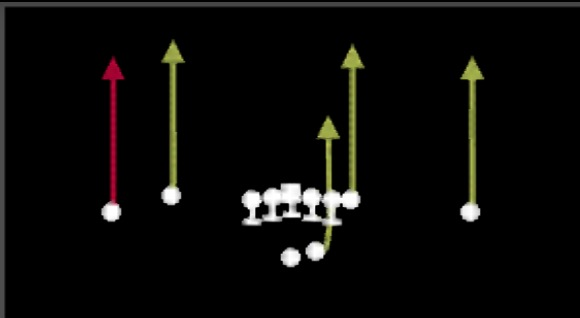
\includegraphics[width=7cm]{figure/hailMary.png}
    \caption{A depiction of a Hail Mary Pass in video game NFL Mobile.}
\end{figure}

\subsubsection{One Dimension}

\quad While football is a two-dimensional game, we are able to simplify the model into one dimension: the y-dimension. This simplification is due to the Hail Mary play relying on straight line movement up the field. This model is easily scalable to two dimensions, as the Quarterback only gets safer with more passing and maneuvering options. Furthermore, you can see that the Hail Mary play is roughly symmetric, so modelling it in a single y-dimension, would serve as an important stepping stone to modelling multiple instances of Wide Receivers. The proof would be very similar as the one-dimension case, just along different points of the x-axis.

\subsubsection{The Equivalence of Openness and Passing}

\quad One assumption that we will make is that openness is equivalent to passing. The main problem we seek to discuss is whether our Quarterback safely pass the ball? As such, we will assume that, when presented with the opportunity, our Quarterback will pass the ball to the Wide Receiver as soon as he becomes open. This means that our system has successfully protected the Quarterback for the necessary duration. As such, we will not worry about the physical act of passing for our model since we are focusing on the safety of the Quarterback. Though it is a bit unrealistic to say that the Quarterback can instantaneously pass the ball to the Wide Receiver, we will use this assumption to simplify our model and put a larger focus on Quarterback safety. 

\subsection{Realistic Magnitudes}

\quad Some things we will need to keep in mind for our model are realistic conditions. We are able to set these values and not leave them up to further generality because football is "defined" to have some of these constraints. The first will be the dimensions of the football field, and the speeds of the players. 

\subsubsection{Player Speeds}

\quad We gathered data from the NFL Combine (an event where prospective football players participate in various events to demonstrate their physical abilities) to determine appropriate speeds for our various players [1]. A 40 yard dash time is how long it takes a player to run 120 feet at a full sprint. Note that Quarterbacks usually move slowly since they need to be in a stable position to throw far distances. We model this by setting the QB's speed to the average pace at which a human walks. To get their speed in feet per second we do $120 \div dash$. Since we have this notion of a categorical player, we can reduce each player to their positions and find statistics per positions (Table 1). 

\newpage

\begin{table}[h]
    \centering
    \begin{tabular}{ |c|c|c| } 
     \hline
     \textbf{Position}\footnotemark & \textbf{40-yard Dash Time} & \textbf{Feet Per Second} \\ 
     \hline
     Quarterback & -- & 4.6 \\ 
     Wide Receiver & 4.48 & 26.79 \\ 
     Linebacker & 4.76 & 25.21 \\ 
     Defensive Lineman & 5.06 & 23.71 \\ 
     Offensive Lineman & 5.34 & 22.47 \\ 
     \hline
    \end{tabular}
    \caption{Times from the NFL Combine}
\end{table}


\footnotetext{Here we refer to specifically the Inside Linebacker. Defensive Lineman can also be called Defensive Tackles. finally, The Offensive Lineman is the average of the Offensive Guard and Tackle.}

\subsubsection{The Football Field}

\quad The football field’s dimensions are 160 feet by 300 feet. If we consider the football field to be on a coordinate plane, with the units being in feet, we will let the lower left corner be at the point (0, 0), the upper right corner be at (160, 300), and the center be at (80, 150). We will also consider the scenario where the Quarterback starts at this halfway point in our model (Figure 2).

\begin{figure}[htp]
    \centering
    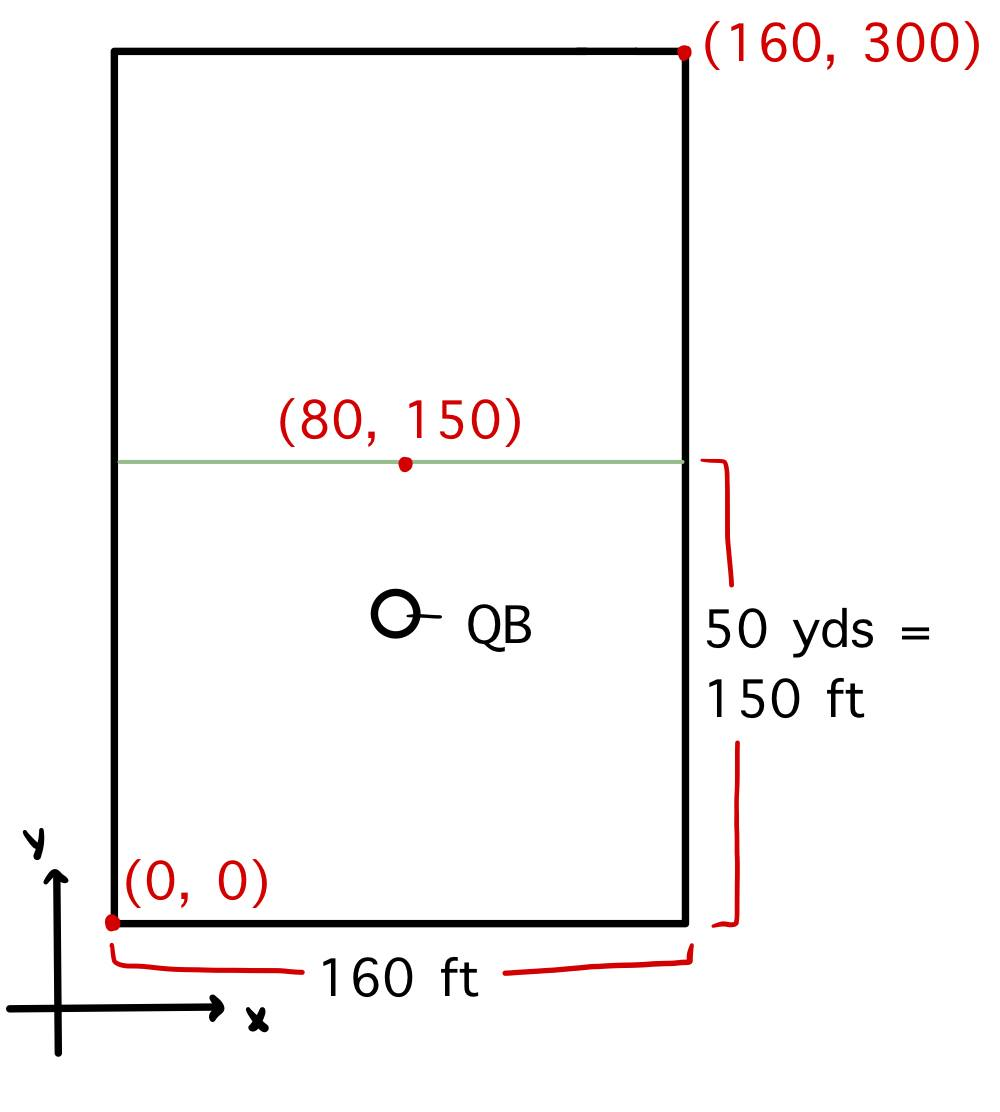
\includegraphics[width=5cm]{figure/1_dimensions.jpg}
    \caption{Geometrical dimensions of a NFL football field}
\end{figure}

\subsection{The Players}

\quad We will break the system down into its smaller subparts, by first examining how the Offensive and Defensive Lines work. To simplify the system, we will consider the Offensive Line and Defensive Line as their own single lines that move as a unit rather than individual players. In real football, the players might struggle to break past one another. For our model, we will simplify this by saying that the Defensive Line slowly approaches the Quarterback.

\subsubsection{Linemen Collision}
\quad  In football, there is no fixed rule as to where the Offensive and Defensive Lines need to start exactly. The only constraint is that the Offensive Line starts in front of the Quarterback on one side of the Line of Scrimmage and the Defensive Line starts on the other side of the Line of Scrimmage as visible in the visual. We will be viewing the football field from the perspective of the offense. \\

Note that the Offensive Line’s duty is to protect the Quarterback and the Defensive Line’s goal is to tackle the Quarterback before he throws the ball. Therefore the Defensive Line travels toward the Quarterback, which is the negative direction on the y-axis ($dy_D$). On the other hand, the Offensive Line travels away from the Quarterback, which means they travel in the positive direction on the y-axis ($dy_A$). To simplify the model, we consider that both of the lines travel with a constant velocity before they collide. We visualize the velocities and directions of the two lines in the following diagram (Figure 3). \\

\begin{figure}[htp]
    \raisebox{-0.08\height}{
    \hspace*{1.75cm}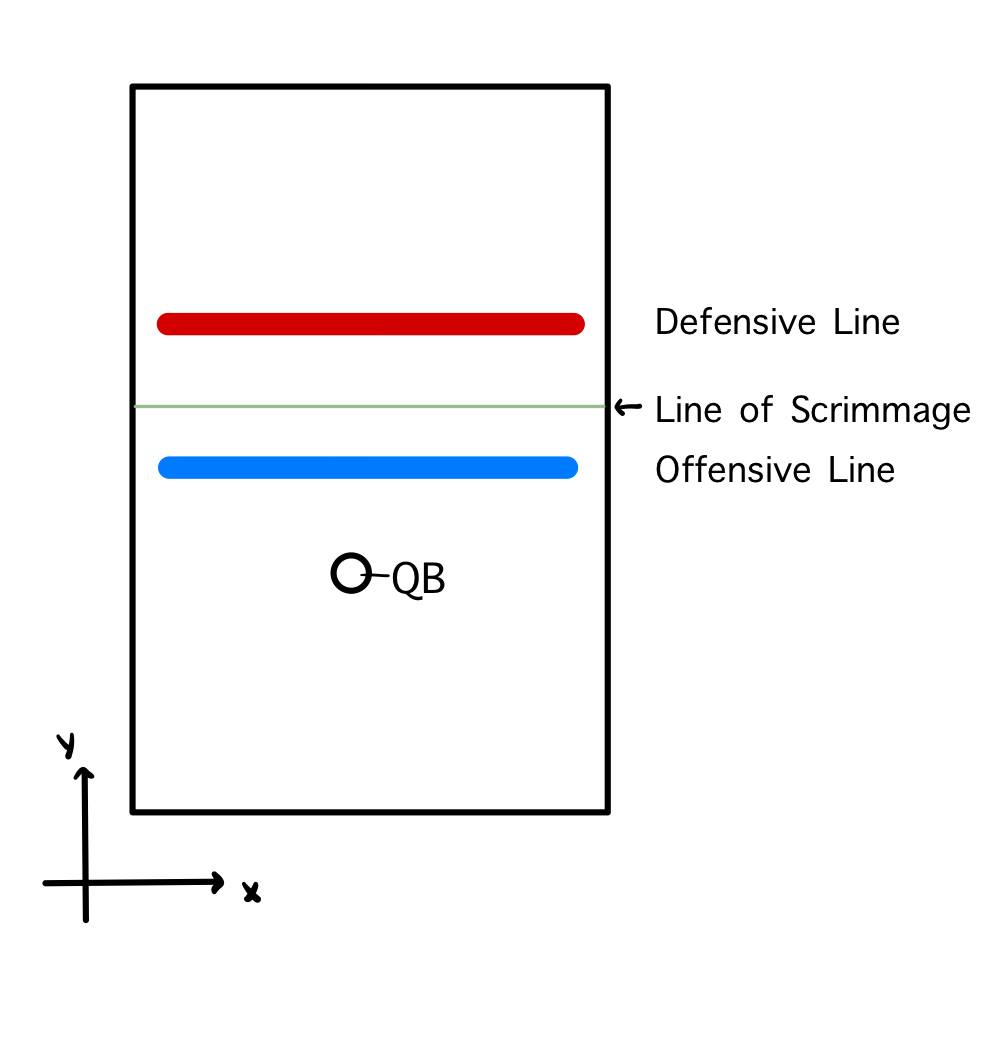
\includegraphics[width=6.62cm]{figure/2_line_layout.jpg}
    }
    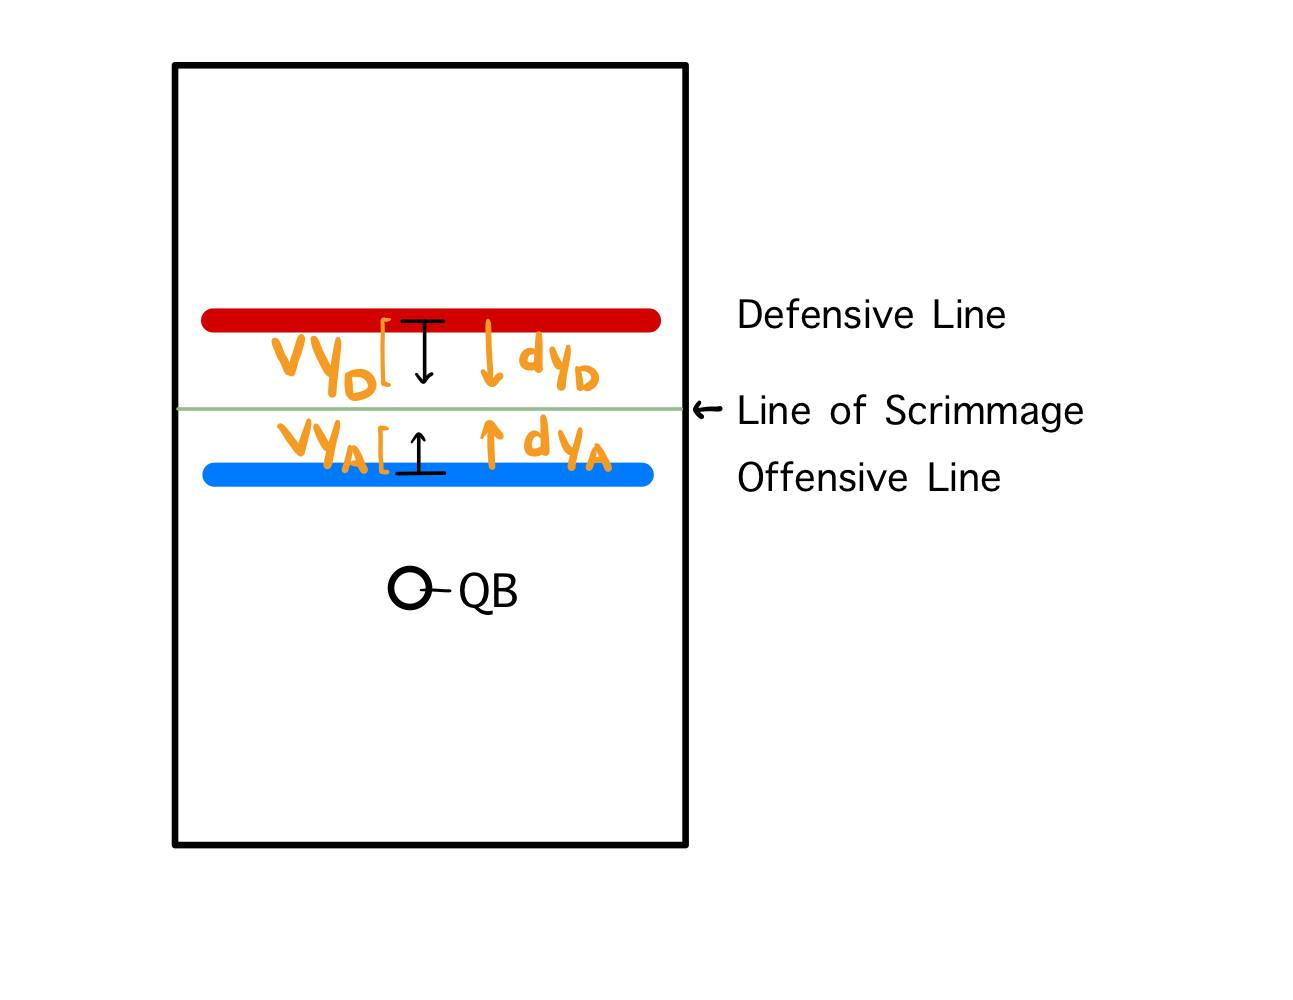
\includegraphics[width=7.8cm]{figure/3_line_velocities.jpg}
    \caption{Layout of Offensive and Defensive Lines}
\end{figure}

The Defensive Line, represented by the red line, is moving with speed $vy_D$ in the direction $dy_D$, and the Offensive Line (blue) is moving with speed $vy_A$ in direction $dy_A$. Note that $vy_D$ and $vy_A$ are the magnitudes of the lines' velocities, and are therefore non-negative. 

\newpage
 
At the start of the play, the two lines will charge towards each other. However, once the two lines collide, they will move as one unit with the velocity being the sum of their initial velocities; this models a perfectly inelastic collision. From \textbf{3.2 Realistic Magnitudes}, we see that Defensive Linemen are on average faster than Offensive Linemen; we model this by making the magnitude of the initial velocity of the Defensive Line greater than the magnitude of the velocity of the Offensive Line. Therefore, when the two lines collide, their velocities will counteract one another, effectively dampening the velocity of the Defensive line. \\

One might think of this as two people pushing against one another, but one eventually dominating the other in terms of force, thus pushing them back. Taking into account the force of the Offensive and Defensive lines, we see that they will travel with a velocity that has a magnitude equivalent to half of the difference between the magnitudes of the initial Defensive and Offensive Line’s velocities. If we consider that the masses of the Offensive and Defensive Lines are the same, we know that this abides with the Principle of Momentum Conservation because of the following equations. \\

Let $m_A$ and $m_D$ be the masses of the Offensive and Defensive lines respectively, where $m_A = m_D = m$. Let $vy_{Ai}$ and $dy_{Ai}$ be the initial velocity (magnitude) and direction of the Offensive Line, $vy_{Di}$ and $dy_{Di}$ be the initial velocity (magnitude) and direction of the Defensive Line, and $vy_f$ and $dy_f$ be the final velocity and direction of both lines together after the collision. By the conservation of momentum, we have:
% Len: I changed this slightly because things are showing up weird on Overleaf
\begin{align*}
m_A \cdot vy_{Ai} \cdot dy_{Ai} + m_D \cdot vy_{Di} \cdot dy_{Ai} &= m_A \cdot vy_f \cdot dy_f + m_D \cdot vy_f \cdot dy_f \\
m(vy_{Ai} \cdot dy_{Ai} + vy_{Di} \cdot dy_{Ai}) &= 2 \cdot m \cdot vy_f \cdot dy_f & (m = m_A = m_D) \\
m(vy_{Ai} - vy_{Di}) &= 2 \cdot m \cdot vy_f \cdot dy_f & (vy_{Ai} = 1, vy_{Di} = -1) \\
vy_{Ai} - vy_{Di} &= 2 \cdot vy_f \cdot dy_f & (\text{eliminate m}) \\
\frac{vy_{Ai} - vy_{Di}}{2} &= -vy_f
\end{align*}

Since $vyDi > vyAi$ (the Defensive Line is faster than the Offensive Line), we know that the left hand side has to be negative as $\frac{vyAi - vyDi}{2} < 0$. Therefore, $vyf \cdot dyf < 0$, and $vyf$ is a magnitude so it cannot be negative. Therefore, $dyf = -1$, and the direction is the same as the Defensive Line’s original direction. We have $\frac{vyAi - vyDi}{2} = -vyf$. The progression of movement is shown in Figure 4.

\newpage

\begin{figure}[htp]
    \centering
    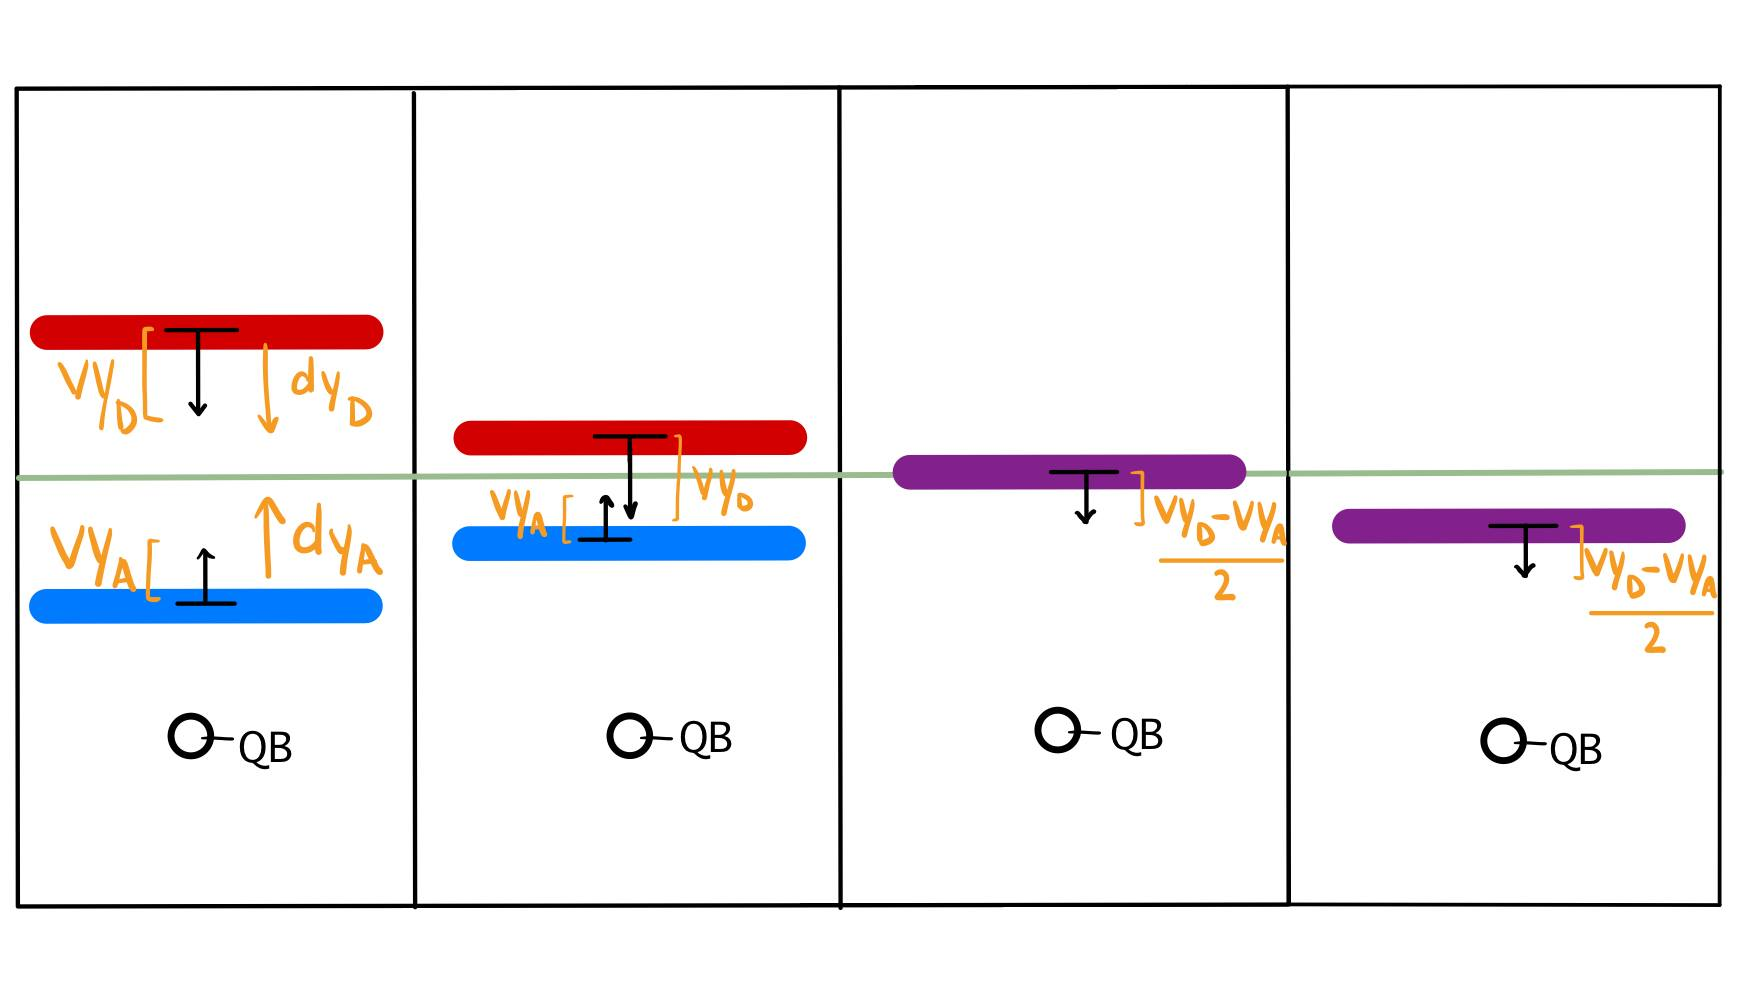
\includegraphics[width=12.5cm]{figure/4_line_evolution.jpg}
    \caption{Evolution of Offensive and Defensive Lines}
\end{figure}

\subsubsection{The Quarterback and Wide Receiver} % subsubsection of "the players"

\quad In football, the Quarterback is the player who passes the ball, so he has great control over how the offensive play is conducted. In order for us to successfully advance the ball up the field, it is essential for the Quarterback to remain safe enough to pass to the Wide Receivers. This requires that the Quarterback does not get tackled by the Defensive Line until he executes a pass. Recall from \textbf{1.3 Football Through The Lens of Hybrid Systems}, tackling is represented as the intersection of their y-coordinates. The winning strategy is dependent on two things: the Quarterback’s ability to both pass and stay away from the Defensive Line. \\

The Quarterback is able to avoid a collision with the Defensive Line by moving away from it. In this scenario, "away" would mean moving backwards from the Defensive Line. We also know that the Quarterback's speed is faster than the dampened Defensive Line speed, so his safety is ensured. Therefore, the only aspect remaining to ensure a successful run is whether the Wide Receiver can get open while all the players are still on the field. From \textbf{3.1.4 The Equivalence of Openness and Passing}, the Quarterback will pass as soon as the Wide Receiver is open. However, this notion of openness will be different in certain scenarios. We partition these scenarios into two defensive strategies, or their more colloquially known terms: "man" and "zone." 

\newpage

\subsubsection{Man Defense}

% Added by Len
\quad Recall that a "man-to-man", or "Man", defense is one where each Linebacker tightly guards a Wide Receiver. Since our model has been reduced to categorical players, this means that our Linebacker will start as close as he can to the Wide Receiver. As we will later formalize in \textbf{4.3 Preconditions}, this closest distance is the Line of Scrimmage. As such, our singular Linebacker will likely start where the Defensive Line starts as well. \\

% Added by Len
Since the Linebacker will be able to closely follow the Wide Receiver for the majority duration of his evolution (or his act of running forward), the Wide Receiver will only be open if he runs past the Linebacker. Within the context of our model, the Wide Receiver will become open if his y-coordinate is greater than the y-coordinate of the Linebacker. However, this relies on the speed of the Wide Receiver being greater. From earlier, we reasoned that the difference in speed between the two is rather small. This small difference thus requires a long distance or great amount of time in order for the Wide Receiver to "run past" the Linebacker. We will see later that this becomes very difficult to prove without using blatantly unrealistic preconditions.

\subsubsection{Zone Defense}

\quad Recall that a Zone Defense is one where the defensive players attempt to spread themselves out evenly throughout the field to cover all "zones", hence the name. For our model, this means that the Linebacker will start at some evenly spread distance behind the Defensive Line, which we will later formalize as roughly the halfway point between the Line of Scrimmage and the end of the field. The difference now is that there is a "healthy chunk" of distance between where the Wide Receiver and Linebacker starts. For our Quarterback, the decision to pass now suddenly flips. Instead of waiting for our Wide Receiver to run past the Linebacker like before, we now, we want to pass it before the Linebacker gets a chance to come down the field and tackle him. Notice that this means that the direction our Linebacker is traveling is flipped to the other direction, as is our notion of "openness". \\

We will show that this scenario is preferable for Quarterback safety. While in a Man defense scenario, we have a chance to pass it further and advance the ball down the field an even greater magnitude (in a sense having our controller be "more efficient"), this will be at the cost of compromising the safety of our Quarterback. In a Zone defense, while the distance which the ball moves forward may be less, our Quarterback will be provably safe. Through the lens of a hybrid system, this is much more desirable.
 % Adds your theory section 
%----------------------------------------------------------------------------------------
% Actual Keymaera model
%----------------------------------------------------------------------------------------

\section{Model}

\subsection{Definitions}

\blindtext

\begin{lstlisting}
Definitions

 Real Diff = 2; /* maximum difference in faceups between OL/DL or WR/LB */
 Real T = 40; /* time bound of a play, 40 seconds */

 /* Direction of velocity in y-direction */
 Real dyQB = -1; /* quarterback goes down */
 Real dyA = 1; /* offensive line goes up */
 Real dyD = -1; /* defensive line collides against OL (down) */
 Real dyWR = 1; /* wide receiver goes up */
 /* Real dyLB = 1; /* line backer follows wide receiver (up) Strat Bad */
 Real dyLB = -1; /* line backer follows wide receiver (down) Strat Good */

 /* Helper Functions */
 Bool onField(Real y) <-> 0 <= y & y <= 300; /* Player is on the field */
 /* Bool isOpen(Real yWR, Real yLB, Real buffer) <-> yLB + buffer < yWR; /* WR ran past LB */
 Bool isOpen(Real yWR, Real yLB, Real buffer) <-> yWR + buffer < yLB; /* WR not yet tackled by LB */

End.
\end{lstlisting}

\subsection{Program Variables}

\blindtext

\begin{lstlisting}
ProgramVariables

 Real diffLine; /* Difference in the speed of offernsive and defensive line */
 Real diffPass; /* Difference in the speed of wide receiver and linebacker */

 Real buffer; /* y- position buffer for WR/LB */

 Real yQB; /* y-position of the quarterback (Angel-team) */
 Real vyQB; /* magnitude of velocity in y-direction of the quarterback */

 Real yA; /* y-position of the offensive line (Angel-team) */
 Real vyA; /* magnitude of velocity in y-direction of the offensive line */

 Real yD; /* y-position of the defensive line (Demon) */
 Real vyD; /* magnitude of velocity in y-direction of the defensive line */

 Real yWR; /* y-position of the wide receiver (Angel-team) */
 Real vyWR; /* magnitude of velocity in y-direction of the wide receiver */

 Real yLB; /* y-position of the linebacker (Demon-team) */
 Real vyLB; /* magnitude of velocity in y-direction of the linebacker */

 Real t; /* Running time of the play*/

End.
\end{lstlisting}

\subsection{Problem}

\blindtext

\begin{lstlisting}
Problem
  ( yQB = 150 /* Quarterback starts at half way point */
  & yA = yQB + 15 /* OL starts 5 yards above QB */
  & yD = yA + 3 /* DL starts 1 yard above OL */
  & yWR = yA /* Start at line of scrimmage with OL */
  /*& yLB = yD /* Start at line of scrimmage with DL (Strat Bad) */
  & yLB = (yD + 300) / 2 /* Start at safe distance (Strat Good) */
  & 0 < diffLine & diffLine < Diff /* offset the OL/DL */
  & 0 < diffPass & diffPass < Diff /* offset the WR/LB */
  & buffer = 0
  & vyQB = 4.6 /* Walking speed in ft/s */
  & vyD  = 23.72 /* Avg for DL in ft/s from combine */
  & vyWR = 26.79 /* Avg for WR in ft/s from combine */
  ) ->
  <
    vyA  := vyD  - diffLine; /* OL's strength/velocity is always less than DL's */
    vyLB := vyWR - diffPass; /* LB's strength/velocity is always less than WR's */
    t:= 0;

    /* Pre-collision movement, ball getting "hiked" */
    { yQB' = dyQB*vyQB,
      yA'  = dyA*vyA,
      yD'  = dyD*vyD,
      yWR' = dyWR*vyWR,
      yLB' = dyLB*vyLB,
      t' = 1
      & yA <= yD /* Pre-collision */
      & t <= T /* Realism */
    }

    /* Keep evolving; stop once WR open or realism breaks */
    { yQB' = dyQB*vyQB,
      yD'  = (dyA*vyA + dyD*vyD)/2, /* Dampened Movement */
      yWR' = dyWR*vyWR,
      yLB' = dyLB*vyLB,
      t' = 1
    & yA >= yD /* Collided */
    & t <= T /* Realism */
    }

  >( yQB < yD /* QB unhurt */
   & isOpen(yWR, yLB, buffer) /* Passed (assuming pass <=> open) */
   & onField(yQB) & onField(yD)
   & onField(yWR) & onField(yLB)
   & t <= T /* Within 40 second play clock */
   )
End.
End.
\end{lstlisting}

 % Adds your model
\newpage

%----------------------------------------------------------------------------------------
% Proof
%----------------------------------------------------------------------------------------

\section{Proof}

\subsection{Diamond Modalities}
\quad In order for the offense to have a successful play, it is not necessary for every possible run of the system to yield a winning strategy. Rather, there simply needs to exist one winning play, and the offense will ideally follow that play regardless of how the defense behaves. Therefore, a diamond modality is much more suited for the purpose of modeling a football play. It follows almost directly, that we can use differential game logic to define a winning strategy, by allowing the defense to make a few non-deterministic choices using the dual operator. Interestingly, in differential game logic, finding and proving a winning strategy for the offense is very similar to modeling the play as a diamond modality. \\

While in past work we have utilized box modalities to represent safety and efficiency for all possible runs of a hybrid system, utilizing a diamond modality allows for some different modeling heuristics. In this section we will discuss how we can take advantage of the diamond modality. \\

One of the subtleties of box modalities was the domain constraint of differential equations. Since box modalities are meant to show that all possible runs of a system are safe and efficient, one could not blatantly violate physics. In other words, one could not restrict the domain of an ODE simply to prove the post-condition, because in the real world, the domain is not restricted. For example, in the case of proving a bouncing ball remains within a certain height, one could not restrict the differential equation to only run while the ball’s height is safe. The model would also have to include the domain which is unsafe for the ball and instead, be able to develop the model such that the ball never travels into the unsafe domain. \\

However, for the diamond modality, restricting physics through domain constraints is viable because we need to show that at least one successful run exists. Essentially, having domain constraints within a diamond modality makes maintaining that domain constraint the responsibility of the offense. We utilized this fact to move the condition that the Quarterback remains unhurt from the post-condition into the domain constraint. In the post-condition, we recognized that the Quarterback could possibly get tackled and then move into safety again, which would still be considered a winning strategy despite being blatantly incorrect. Therefore, we noted that the Quarterback must not be tackled through the entire run of the differential equation.

\subsubsection{Proof Tactics}
\quad Another difference between box and diamond modalities lies in the proof of them. In box modalities, a common proof method for loops was defining a loop invariant which remained true throughout every iteration of the loop. However, for diamond modalities, the post-condition does not have to remain true throughout the entire run. Therefore, we were able to utilize iterating through the loop until we found a successful run. \\

Our other fundamental tactic for finding a proof was utilizing solvable differential equations. Due to this, we were able to use kinematic equations, and solve them to show our post-conditions were satisfied. \\

While we were originally able to utilize the KeYmaera X tool for our proofs, in our third iteration of modeling, we experienced an impediment. Utilizing Mathematica 12.0.0, we were able to prove contradicting models. Let P, represent the formula in our post-condition. In one run, we proved that given a valid pre-condition, there exists a run such that P is true. Then in the other run, we proved that given the same valid pre-condition, for all runs P is not true. These contradictory statements forced us to stop modeling and start proving our models by hand. While this hindered our ability to add more complexities into our model, we are hopeful for future work in this area. 

\subsection{Finding the Time}

\quad One thing that we also did to further convince ourselves of the correctness of our program was to hand write some examples and proofs of our model. Many of our ODE's are solvable with a basic kinematics solution. For example, \texttt{yQB' = dyQB * vyQB} can be solvable as $yQB(t) = dyQB \cdot vyQB \cdot t + yQB_0$ for some initial position. Further elaborated given our preconditions, we can see this as a family-friendly kinematics problem: $yQB(t) = -4.6t + 150$. While solving these, we came across a few interesting observations. Note from kinematics and math we have $t = \frac{x_f - x_0}{v}$ From here, we could use the information from our preconditions to find more meaningful times. Note that according to our model, our quarterback is able to pass anytime between the Lineman Collision and the Wide Receiver becoming open. We can quantify those times in the following way:

\begin{align*}
    T_\texttt{lc} = T_\texttt{lineman collision} &= \frac{\texttt{yD - yA}}{\texttt{dyD * vyD - dyA * vyA}} = \frac{\texttt{yD - yA}}{\texttt{2*vyD - diffLine}} \\
    T_\texttt{zone} = T_\texttt{wr open zone} &= \frac{\texttt{yLB - yWR}}{\texttt{dyLB * vyLB - dWR * vyWR}} = \frac{\texttt{yLB - yWR}}{\texttt{2*vyWR - diffPass}} \\ 
    T_\texttt{man} = T_\texttt{wr open man} &= \frac{\texttt{yWR - yLB}}{\texttt{dWR * vyWR - dyLB * vyLB}} = \frac{\texttt{yWR - yLB}}{\texttt{2*vyWR - diffPass}} \\
\end{align*}
Since we define the speed of \texttt{yA} and \texttt{yLB} relative to their pairings (\texttt{yD, yWR}), we can substitute their values to simplify the velocity quantities as seen above. If $T$ represents the critical point, then in a sense we can also note that $\forall t \le T_{\texttt{zone}}, \texttt{isOpen(WR,LB,buffer) <-> true}$ since the Wide Receiver is open until he gets tackled by the Linebacker in a Zone defense. We also see that $\forall t \ge T_{\texttt{man}}, \texttt{isOpen(WR,LB,buffer) <-> true}$ since the Wide Reciever is not open until he gets past the Linebacker in a Man defense. The reason we mention all this time, is that we can view the proof of our model as a simple question. Do I have time to pass? Is there a time after lineman collision that the wide receiver is open for a sufficient amount of time? While this is not how \texttt{KeymaeraX} does the proof, it helped us better understand what was going on and verify it to ourselves, that in a way, we could think of our model as the following statement: $\exists t \text{ such that } T_{\texttt{ lineman collision }} < t < T_{\texttt{open}}$. \\

One aspect, however, that this handwritten logic does not cover is realism: we might find a time that we can pass, but can we ensure that the players are still on the field when this happens? Fortunately we have \texttt{KeymaeraX} to double check us on that. Regardless, thinking about this helped us better convince ourselves of the \texttt{KeymaeraX} proof tactic.  % Adds your proof
\newpage

%----------------------------------------------------------------------------------------
% Future
%----------------------------------------------------------------------------------------

\section{Future Considerations}

\subsection{Quarterback Controller}

\quad While we faced some trouble moving onto the next iteration of our model, in our future work we plan to add more complexity to the Quarterback’s controller. This includes finishing the implementation of forward and backwards movement, so that the Quarterback can move more freely. This includes a loop which starts with a control that switches direction based on conditions that include how far the wide receiver is and how far the defensive line is. Recall that a winning strategy for the offense requires both the wide receiver and the defensive line. \\

Another continuation of this model would be to define a maximum passing range for the Quarterback, because currently, the Quarterback passes as soon as the Wide Receiver is open. The average Quarterback can only throw between 70 to 80 yards, so it is not entirely realistic if the Quarterback is at yard 0 and passed to the Wide Receiver at yard 100. Our constraint on the Quarterback and Wide Receiver would be that they are within 200 feet of each other. To calculate the distance, we would simply subtract their y-coordinates. However, when we move into two dimensions, as discussed in the next section this distance would be the Euclidean distance between them. \\

To implement this maximum passing range, there are two different notions. One is to allow the Quarterback to travel backwards while he is within 200 feet of the Wide Receiver. While this will allow the Quarterback to avoid getting tackled by the Defensive Line for as long as possible, it may make it harder for the offense to win in the case that he travels too far back and can never reenter a 200 foot range of the Wide Receiver. Therefore, the other notion is to allow the Quarterback to travel backwards while he is within half of the 200 foot range. That way, it is more likely that once the Wide Receiver gets open that the Quarterback will still be in the range to throw the ball. However, this constraint also makes it harder for the Quarterback to avoid getting tackled by the Defensive Line. Both notions have their pros and cons, so we would test both out. \\

\subsection{Two Dimensions}

\quad While football is a two-dimensional game, as players move in the x and y direction, we were able to simplify the model into one dimension, the y-dimension, due to the Hail Mary play being predominantly vertical. However, it is indeed more realistic to allows players, like the Wide Receiver, Quarterback, and Linebacker to travel in the x-direction. \\

Therefore, in the future, we would start by introducing the x-direction for the Wide Receiver to enable movement around the Linebacker. Then, we would introduce the x-direction to the Linebacker’s controllers to model defending the Wide Receiver more accurately. The final step would be integrating a controller in the x-direction for the Quarterback to enable getting closer to the Wide Receiver in the x-direction, so as to remain within 200 feet of him. This last step relates back to offense’s ability to win, because the Quarterback would have a constraint on how far he could throw.

\subsection{Different Defensive Line}

\quad Currently, our Offensive and Defensive Lines' actions are modelled as a dampened line moving slowly towards the Quarterback. If we want to make this even more realistic, we would want to model the scenario that an additional linebacker or one of the linemen are able to get past the offensive line. In this scenario, we would see a sack happen, where the quarterback gets tackled before he gets a chance to pass it, or behind the line of scrimmage. One way we could model this is, assuming we modelled multiple linemen individually instead of as a "collective", is choose with some random probability one player to "break past". 

Going off the idea of multiple linemen, another thing we would want to consider is modelling a curve. Generally you'll see that linemen are not an exact straight line, but rather a curve: the outside more curved than the inside. This is because they all have the common goal of tackling the quarterback and likely will take the shortest distance to accomplish that, instead of moving directly forward. However, since our model is one dimensional, a straight line sufficed for our problem. % Adds your future discussion
%----------------------------------------------------------------------------------------
% Partner
%----------------------------------------------------------------------------------------

\section{Per Partner}

Equal work was done by both partners.
 % Adds your partner
\newpage

%----------------------------------------------------------------------------------------
% Conclusion
%----------------------------------------------------------------------------------------

\section{Conclusion}

\blindtext % Some blind text
 % Adds your conclusion
%----------------------------------------------------------------------------------------
% Bibliography
%----------------------------------------------------------------------------------------
\newpage % Includes a new page

% \pagenumbering{roman} % Changes page numbering to roman page numbers
%\bibliography{literature}

\section{References}

% \bibliography{literature.bib} % Add the filename of your bibliography
% \bibliographystyle{apsr} % Defines your bibliography style

% For citing, please see this sheet: http://merkel.texture.rocks/Latex/natbib.php



[1] Doll, T. (2013, February 12). Some Clarification is in Order: Average Speed by Position. Retrieved November 29, 2020, from \\ https://www.milehighreport.com/2013/2/12/3969128/some-clarification-is-in-order-average-speed-by-position \\
 
[2] Dudek, G., Jenkin, M. R., Milios, E., \& Wilkes, D. (1996). A taxonomy for multi-agent robotics. Autonomous Robots, 3(4), 375-397. \\
http://citeseerx.ist.psu.edu/viewdoc/download?doi=10.1.1.57.621\&rep=rep1\&type=pdf \\
 
[3] Gaines, C. (2016, February 07). Cam Newton's emergence will change what quarterbacks look like in the NFL. Retrieved November 29, 2020, from \\ https://www.businessinsider.com/cam-newton-is-big-2016-2 \\
 
[4] Operations, N. (n.d.). Evolution of the NFL Player. Retrieved November 29, 2020, from \\ https://operations.nfl.com/the-players/evolution-of-the-nfl-player/ \\
 
[5] Platzer, A. (2010, August). Quantified differential dynamic logic for distributed hybrid systems. In International Workshop on Computer Science Logic (pp. 469-483). Springer, Berlin, Heidelberg.
\\ http://symbolaris.com/pub/QdL.pdf  \\
 
[6] Platzer A., Clarke E.M. (2009) Formal Verification of Curved Flight Collision Avoidance Maneuvers: A Case Study. In: Cavalcanti A., Dams D.R. (eds) FM 2009: Formal Methods. FM 2009. Lecture Notes in Computer Science, vol 5850. Springer, Berlin, Heidelberg. \\ https://doi.org/10.1007/978-3-642-05089-3\_35 \\
 % Adds your references
%----------------------------------------------------------------------------------------
% Appendix
%----------------------------------------------------------------------------------------
\newpage % Includes a new page
\section{Deliverables} % Stars disable section numbers
% Uncomment if you want to add an "automatic" appendix
% \pagenumbering{Roman} % Changes page numbering to Roman page numbers

\subsection{Proved Model for QB Avoidance of Linemen}

This is one of our earlier models where we started off by just showing that the Quarterback could be safe from the Defensive Line, not considering the Wide Receivers and Linebacker.

\begin{lstlisting}
/* Exported from KeYmaera X v4.9.1 */

Theorem "STAR LAB TRIAL 1"

Definitions

 Real Diff = 2; /* maximum difference in strength of offensive and defensive line*/
 Real T = 40; /* time bound of a play, 40 seconds*/

 Real dyA = 1; /* direction of velocity in y-direction of the offensive line*/
 Real dyD = -1; /* direction of velocity in y-direction of the defensive line*/
 Real dyQB = -1; /* direction of velocity in y-direction of the Quarter Back*/

End.

ProgramVariables

 Real diff; /* Difference in the strength of offensive and defensive line*/

 Real maxVel; /* maximum realistic velocity */

 Real yA; /* y-position of the offensive line (Angel-team)*/
 Real vyA; /* magnitude of velocity in y-direction of the offensive line*/

 Real yD; /* y-position of the defensive line (Demon)*/
 Real vyD; /* magnitude of velocity in y-direction of the defensive line*/

 Real yQB; /* y-position of the Quarter Back (Angel-team)*/
 Real vyQB; /* magnitude of velocity in y-direction of the Quarter Back*/

 Real t; /* Running time of the play*/

End.

Problem
  ( yA = 150 & yD = yA + 3 & yQB = yA - 15
  & maxVel = 24 & vyD = maxVel /* hardcode maxVel for now */
  & 0 < diff & diff < Diff
  & vyQB = 9 ) ->
  <
    vyA := vyD - diff; /* OL's strength/velocity is always less than DL's */
    t:= 0;

    {
      yQB' = dyQB*vyQB, yA' = dyA*vyA, yD' = dyD*vyD, t' = 1
      & yA <= yD & t <= T
    };

    {
      yQB' = dyQB*vyQB, yD' = (dyA*vyA + dyD*vyD)/2, t' = 1
      & yA >= yD & t <= T
    }
  >( yQB < yD
     /* (Ball Not Passed -> yQB < yD) or (Ball Passed -> Ball Caught) */
     /* & 0 <= yA & yA <= 300 angel still on the field */
   & 0 <= yD & yD <= 300 /* demon still on the field */
   & 0 <= yQB & yQB <= 300 /* QB still on the field */
   )
End.

Tactic "STAR LAB TRIAL 1: Proof"
expandAllDefs ; unfold ; assignd(1) ; composed(1) ; solve(1) ; solve(1.0.1.1.0.1.0.1.0.1) ; auto
End.

End.
\end{lstlisting}

\newpage

\subsection{Proved Model for Zone Defense}
Here is our proved model containing both linemen collision and passing in a Zone defense. This was also discussed in \textbf{4 Model}.

\begin{lstlisting}
/* Exported from KeYmaera X v4.9.2 */

Theorem "STAR LAB TRIAL 2"

Definitions

 Real Diff = 2; /* maximum difference in faceups between OL/DL or WR/LB */
 Real T = 40; /* time bound of a play, 40 seconds */

 /* Direction of velocity in y-direction */
 Real dyQB = -1; /* quarterback goes down */
 Real dyA = 1; /* offensive line goes up */
 Real dyD = -1; /* defensive line collides against OL (down) */
 Real dyWR = 1; /* wide receiver goes up */
 Real dyLB = -1; /* line backer follows wide receiver (down) (Zone) */

 /* Helper Functions */
 Bool onField(Real y) <-> 0 <= y & y <= 300; /* Player is on the field */
 /* Bool isOpen(Real yWR, Real yLB, Real buffer) <-> yLB + buffer < yWR; /* (Man) */
 Bool isOpen(Real yWR, Real yLB, Real buffer) <-> yWR + buffer < yLB; /* (Zone) */

End.

ProgramVariables

 Real diffLine; /* Difference in the speed of offensive and defensive line */
 Real diffPass; /* Difference in the speed of wide receiver and linebacker */

 Real buffer; /* y-position buffer for WR/LB */

 Real yQB; /* y-position of the quarterback (Angel-team) */
 Real vyQB; /* magnitude of velocity in y-direction of the quarterback */

 Real yA; /* y-position of the offensive line (Angel-team) */
 Real vyA; /* magnitude of velocity in y-direction of the offensive line */

 Real yD; /* y-position of the defensive line (Demon) */
 Real vyD; /* magnitude of velocity in y-direction of the defensive line */

 Real yWR; /* y-position of the wide receiver (Angel-team) */
 Real vyWR; /* magnitude of velocity in y-direction of the wide receiver */

 Real yLB; /* y-position of the linebacker (Demon-team) */
 Real vyLB; /* magnitude of velocity in y-direction of the linebacker */

 Real t; /* Running time of the play*/

End.

Problem
  ( yQB = 150 /* Quarterback starts at half way point */
  & yA = yQB + 15 /* OL starts 5 yards above QB */
  & yD = yA + 3 /* DL starts 1 yard above OL */
  & yWR = yA /* Start at line of scrimmage with OL */
  & yLB = (yD + 300) / 2 /* Start at safe distance (Zone) */
  & 0 < diffLine & diffLine < Diff /* offset the OL/DL */
  & 0 < diffPass & diffPass < Diff /* offset the WR/LB */
  & buffer = 0
  & vyQB = 4.6 /* Walking speed in ft/s */
  & vyD  = 23.72 /* Avg for DL in ft/s from combine */
  & vyWR = 26.79 /* Avg for WR in ft/s from combine */
  ) ->
  <
    vyA  := vyD  - diffLine; /* OL's strength/velocity is always less than DL's */
    vyLB := vyWR - diffPass; /* LB's strength/velocity is always less than WR's */
    t:= 0;

    /* Pre-collision movement, ball getting "hiked" */
    { yQB' = dyQB*vyQB,
      yA'  = dyA*vyA,
      yD'  = dyD*vyD,
      yWR' = dyWR*vyWR,
      yLB' = dyLB*vyLB,
      t' = 1
      & yA <= yD /* Pre-collision */
      & t <= T /* Realism */
    }

    /* Keep evolving; stop once WR open or realism breaks */
    { yQB' = dyQB*vyQB,
      yD'  = (dyA*vyA + dyD*vyD)/2, /* Dampened Movement */
      yWR' = dyWR*vyWR,
      yLB' = dyLB*vyLB,
      t' = 1
    & yA >= yD /* Collided */
    & t <= T /* Realism */
    }

  >( yQB < yD /* QB unhurt */
   & isOpen(yWR, yLB, buffer) /* Passed (assuming pass <=> open) */
   & onField(yQB) & onField(yD)
   & onField(yWR) & onField(yLB)
   & t <= T /* Within 40 second play clock */
   )
End.

Tactic "STAR LAB TRIAL 2: Proof"
expandAllDefs ; unfold ; assignd(1) ; composed(1) ; solve(1.1) ; solve(1) ; QE
End.

End.
\end{lstlisting}

\newpage

\subsection{QB Controller and dGL}

Here is an unproved model that has many ideas we discussed in \textbf{Future Considerations}. The main additions include a nonzero buffer, game logic for the speed assignment, and a loop based QB controller.

\begin{lstlisting}
ArchiveEntry "STAR LAB TRIAL 3"

Definitions

 Real Diff = 2; /* maximum difference in faceups between OL/DL or WR/LB */
 Real T = 40; /* time bound of a play, 40 seconds */
 Real maxPass = 100; /* Passing Heuristic */
 /* Real maxPass = 200; /* Restriction on physics */

 /* Direction of velocity in y-direction */
 Real dyA = 1; /* offensive line goes up */
 Real dyD = -1; /* defensive line collides against OL (down) */
 Real dyWR = 1; /* wide receiver goes up */
 Real dyLB = 1; /* line backer follows wide receiver (up)*/

 /* Helper Functions */
 Bool onField(Real y) <-> 0 <= y & y <= 300; /* Player is on the field */
 /* Bool isOpen(Real yWR, Real yLB, Real buffer) <-> yLB + buffer < yWR; /* (Man) */
 Bool isOpen(Real yWR, Real yLB, Real buffer) <-> yWR + buffer < yLB; /* (Zone) */
 Real dist(Real a, Real b) = abs(a - b); /* 1 dimension, just diff in pos*/

End.

ProgramVariables

 Real diffLine; /* Difference in the speed of offensive and defensive line */
 Real diffPass; /* Difference in the speed of wide receiver and linebacker */

 Real buffer; /* y- position buffer for WR/LB */

 Real yQB; /* y-position of the quarterback (Angel-team) */
 Real vyQB; /* magnitude of velocity in y-direction of the quarterback */
 Real dyQB; /* quarterback goes down */

 Real yA; /* y-position of the offensive line (Angel-team) */
 Real vyA; /* magnitude of velocity in y-direction of the offensive line */

 Real yD; /* y-position of the defensive line (Demon) */
 Real vyD; /* magnitude of velocity in y-direction of the defensive line */

 Real yWR; /* y-position of the wide receiver (Angel-team) */
 Real vyWR; /* magnitude of velocity in y-direction of the wide receiver */

 Real yLB; /* y-position of the linebacker (Demon-team) */
 Real vyLB; /* magnitude of velocity in y-direction of the linebacker */

 Real t; /* Running time of the play*/

End.

Problem
  ( 0 <= yQB & yQB <= 150 /* Quarterback is in the back half of the field */
  & yA = yQB + 15 /* OL starts 5 yards above QB */
  & yD = yA + 3 /* DL starts 1 yard above OL */
  & yWR = yA /* Start at line of scrimmage with OL */
  & yLB = yD /* Start at line of scrimmage with DL (Man) */
  /* yLB = (yD + 300) / 2/* Start back (Zone) */
  & 0 < diffLine & diffLine < Diff /* offset the OL/DL */
  & 0 < diffPass & diffPass < Diff /* offset the WR/LB */
  & vyQB = 9 /* Walking speed in ft/s */
  & vyD  = 15.18 /* Avg for DL in ft/s from combine */
  & vyWR = 13.44 /* Avg for WR in ft/s from combine */
  ) ->
  <
    {
      vyA := *; /* Demon chooses vyA speed to approach QB quicker */
      ?(0 < vyD - vyA & vyD - vyA < diffLine); /* ensure realistic velocity */
      vyLB := *; /* Demon chooses vyLB to best defend against WR */
      ?(0 < vyWR - vyLB & vyWR - vyLB < diffPass); /* ensure realistic velocity */
    }^@

    t:= 0;

    /* Pre-collision movement, ball getting "hiked" */
    { yQB' = dyQB*vyQB,
      yA'  = dyA*vyA,
      yD'  = dyD*vyD,
      yWR' = dyWR*vyWR,
      yLB' = dyLB*vyLB,
      t' = 1
      & yA <= yD /* Pre-collision */
      & t <= T /* Realism */
    };

    {
      /* If within maxPass, move backwards. Else, move forward */
      ?(dist(yQB, yWR) <= maxPass); dyQB := -1; ++ dyQB := 1;

      /* Keep evolving; stop once WR open or realism breaks */
      { yQB' = dyQB*vyQB,
        yD'  = (dyA*vyA + dyD*vyD)/2, /* Dampened Movement */
        yWR' = dyWR*vyWR,
        yLB' = dyLB*vyLB,
        t' = 1
      & yA >= yD /* Collided */
      & !isOpen(yWR, yLB, buffer) /* WR not open */
      & t <= 1 /* Time Triggered */
      & yQB < yD
      }
    }*

  >( yQB < yD /* QB unhurt */
   & isOpen(yWR, yLB, buffer) /* Passed (assuming pass <=> open) */
   & onField(yQB) & onField(yD)
   & onField(yWR) & onField(yLB)
   & t <= T /* Within 40 second play clock */
   )
End.
End.


\end{lstlisting}% Adds an appendix



%---------------------------------------------------------------------------------

\end{document}
